\documentclass[tikz,border=8pt]{standalone}
% Shared look for every TikZ diagram. Load with \input{../../tools/tikz-style.tex}
\usepackage[T1]{fontenc}
\usepackage{lmodern}
\renewcommand{\sfdefault}{lmr}  % diagrams use the same serif as the text
\usetikzlibrary{arrows.meta, positioning, shapes.geometric, calc, fit, backgrounds}
\definecolor{cblue}{HTML}{4C78A8}
\definecolor{corange}{HTML}{F58518}
\definecolor{cgreen}{HTML}{54A24B}
\definecolor{cred}{HTML}{E45756}
\definecolor{cpurple}{HTML}{B279A2}
\definecolor{cgrey}{HTML}{6B6B6B}
\tikzset{
  every picture/.style={font=\sffamily, line width=1.2pt},
  box/.style={draw=#1, fill=#1!12, rounded corners=4pt, align=center, inner sep=7pt, minimum height=1.1cm},
  box/.default=cgrey,
  arrow/.style={-{Stealth[length=3mm]}, draw=cgrey, line width=1.4pt},
  title/.style={font=\sffamily\bfseries\Large},
  note/.style={font=\sffamily\small, text=cgrey, align=center},
}
\AtBeginDocument{\hyphenpenalty=10000 \exhyphenpenalty=10000}

\begin{document}
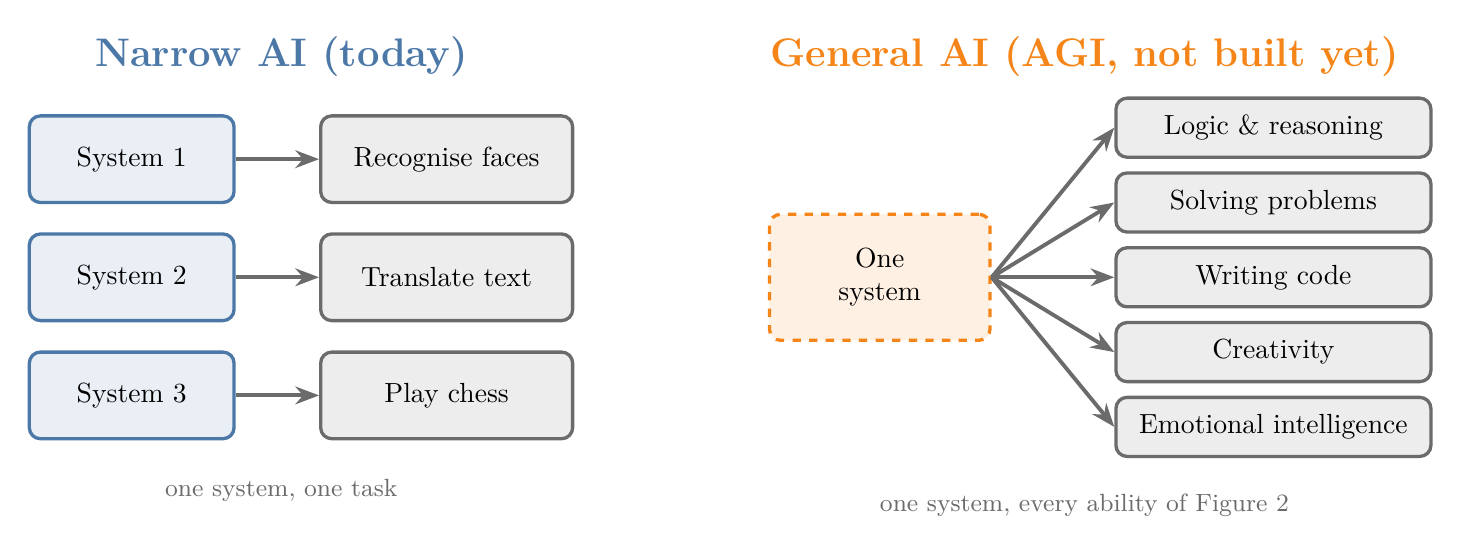
\begin{tikzpicture}
  % narrow AI: one system per task
  \node[title, text=cblue] at (0,3.3) {Narrow AI (today)};
  \foreach \n/\y/\s/\t in {1/2/System 1/Recognise faces, 2/0.5/System 2/Translate text, 3/-1/System 3/Play chess}
    { \node[box=cblue, minimum width=2.6cm] (s\n) at (-1.9,\y) {\s};
      \node[box=cgrey, minimum width=3.2cm] (t\n) at (2.1,\y) {\t};
      \draw[arrow] (s\n) -- (t\n); }
  \node[note] at (0,-2.2) {one system, one task};
  % general AI: one system, every ability
  \node[title, text=corange] at (10.2,3.3) {General AI (AGI, not built yet)};
  \node[box=corange, dashed, minimum width=2.8cm, minimum height=1.6cm] (g) at (7.6,0.5) {One\\system};
  \foreach \n/\y/\t in {1/2.4/Logic \& reasoning, 2/1.45/Solving problems, 3/0.5/Writing code, 4/-0.45/Creativity, 5/-1.4/Emotional intelligence}
    { \node[box=cgrey, minimum width=4cm, minimum height=0.75cm, inner sep=4pt] (a\n) at (12.6,\y) {\t};
      \draw[arrow] (g.east) -- (a\n.west); }
  \node[note] at (10.2,-2.4) {one system, every ability of Figure 2};
\end{tikzpicture}
\end{document}
